\documentclass{standalone}
\usepackage{tikz}
\usepackage{ctex,siunitx}
\usepackage{tkz-euclide}
\usepackage{amsmath}
\usetikzlibrary{patterns, calc}
\usetikzlibrary {decorations.pathmorphing, decorations.pathreplacing, decorations.shapes,}
\begin{document}
\small
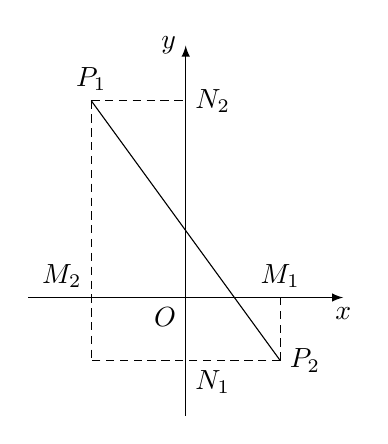
\begin{tikzpicture}[>=latex]
  % \useasboundingbox(0,-0.2)rectangle(3,0.5);
  \draw[thin,->](-2,0)--(2,0)node[below]{$x$};
  \draw[thin,->](0,-1.5)--(0,3.2)node[left]{$y$};
  \node at (0,0)[below left]{$O$};
  \draw(-1.2,2.5)node[above]{$P_1$}--(1.2,-0.8)node[right]{$P_2$};
  \draw[thin,densely dashed](-1.2,2.5)--(0,2.5)node[right]{$N_2$};
  \draw[thin,densely dashed](-1.2,2.5)--(-1.2,0)node[above left]{$M_2$}--(-1.2,-0.8);
  \draw[thin,densely dashed](1.2,-0.8)--(0,-0.8)node[below right]{$N_1$}--(-1.2,-0.8);
  \draw[thin,densely dashed](1.2,-0.8)--(1.2,0)node[above]{$M_1$};
\end{tikzpicture}
\end{document}